\clearpage

\section {Sensitivity to $\nueb$ Appearance}
\label{sec:sensitivity}
Since there are no fitted parameters in the analysis, the validation can be performed by checking for agreement between the oscillation analyses from both the VALOR and P-theta groups. This is done by performing a sensitivity study to $\nueb$ appearance data given the Asimov A data set, which is treated as we would treat the data. The Asimov A data set consists of the most probable data set (obtained by the Bayesian analysis on the T2K run 1-4 neutrino mode data \cite{T2KLongPaper}) that is the nominal expected $E_{reco}$ vs $\theta$ distribution \cite{Asimov} and the corresponding parameters are listed in Tab \ref{tab:osc_params_joint_asimovA}. The expected event rates for all five Super-K event samples using Asimov A parameters are shown in \Crefrange{tab:event_rates_exp_1Rmu}{tab:event_rates_exp_MultiRe}.  %A further check is performed by comparing the distribution of p-values found for \NToysFakeDataRateOnly\ toys data sets.
%TODO: Only uncomment this last sentace if I produce p-value distributions...
%comparing the rate-only with rate+shape p-values and checking if the corresponding distributions are reasonable

%\FloatBarrier

\begin{table}[H]
\centering
\begin{tabular}{| c | c |}
\hline
Parameter(s) 											&	Asimov A 										\\
\hline
$\sin^{2}\theta_{23}$									&	0.528											\\
$\sin^{2} \theta_{13}$ reactors							&	0.0219										\\
$\sin^{2} \theta_{12}$									&	0.304											\\
$|\Delta m^{2}_{32}|$ (NH) / $|\Delta m^{2}_{31}|$ (IH)	&	$2.509 \times 10^{-3}~\mbox{eV}^2/\mbox{c}^4$	\\
$\Delta m^{2}_{21}$										&	$7.53 \times 10^{-5}~\mbox{eV}^2/\mbox{c}^4$	\\
$\delta_{CP}$											&	-1.601											\\
Mass Hierarchy											&	Normal											\\
$\beta$													&   1												\\  
\hline
\end{tabular}
\caption{
Values of oscillation parameters used to compute the event rates, systematic effects and sensitivity studies corresponding to the Asimov A data set, which is the MC expected distribution in a certain oscillation hypothesis.
In the Asimov data set A the nominal values of $\sin^2 2 \theta_{13}$, $\sin^2 2 \theta_{12}$
and $\Delta m^2_{21}$  are from \cite{pdg_2014}, while all the other oscillation parameter values corresponds to the most probable values obtained by the Bayesian analysis on the T2K run 1-4 neutrino mode data \cite{T2KLongPaper}. The mass hierarchy is not marginalised but fixed to either NH or IH.
}
\label{tab:osc_params_joint_asimovA}
\end{table}

%\section*{1Rmu}
\begin{table}
	\centering
	\begin{tabular} { | l ||r | r | r | r | r | r | | r | }
	\hline
	              & $\nu_\mu$            & $\nu_e$              & $\bar{\nu}_{\mu}$    & $\bar{\nu}_{e}$      & Osc. $\nu_e$         & Osc. $\bar{\nu}_{e}$ & Total                \\ \hline\hline
	 CCQE         & 175.69877            & 0.00417              & 11.13658             & 0.00020              & 0.02258              & 0.00015              & 186.86245            \\ \hline
	 CC1pi        & 27.64351             & 0.00201              & 2.64220              & 0.00009              & 0.02418              & 0.00007              & 30.31206             \\ \hline
	 CCcoherent   & 0.28884              & 0.00000              & 0.09306              & 0.00000              & 0.00000              & 0.00000              & 0.38190              \\ \hline
	 2p2h         & 35.49529             & 0.00154              & 1.42670              & 0.00008              & 0.02578              & 0.00004              & 36.94944             \\ \hline
	 CCother      & 5.49849              & 0.00087              & 0.41118              & 0.00008              & 0.00011              & 0.00001              & 5.91073              \\ \hline
	 NC1pi0       & 0.61317              & 0.01856              & 0.02142              & 0.00145              & N/A                  & N/A                  & 0.65460              \\ \hline
	 NC1piPM      & 4.89912              & 0.09882              & 0.17708              & 0.00990              & N/A                  & N/A                  & 5.18492              \\ \hline
	 NCcoherent   & 0.00000              & 0.00000              & 0.00044              & 0.00004              & N/A                  & N/A                  & 0.00047              \\ \hline
	 NCother      & 2.06264              & 0.07441              & 0.13205              & 0.00926              & N/A                  & N/A                  & 2.27837              \\ \hline
	\hline
	 Total        & 252.19982            & 0.20038              & 16.04070             & 0.02110              & 0.07266              & 0.00027              & 268.53493            \\ \hline
	\end{tabular}
	\caption{Predicted number of events in the neutrino mode single-ring $\mu$-like sample obtained after applying the BANFF weight for a total exposure of \TotalPotNuRunOneNineC\ FHC POT. The Asimov data set A in Tab \ref{tab:osc_params_joint_asimovA} is used. The total of 268.53493 events consists of 252.19982 signal events and 16.33511 background events.}
	\label{tab:event_rates_exp_1Rmu}
\end{table}

%Total: 268.53493    (268.53493)
%Total signal: 252.19982
%Total background: 16.33511
%POT: 14.93798E20


%\section*{1Re}
\begin{table}
	\centering
	\begin{tabular} { | l ||r | r | r | r | r | r | | r | }
	\hline
	              & $\nu_\mu$            & $\nu_e$              & $\bar{\nu}_{\mu}$    & $\bar{\nu}_{e}$      & Osc. $\nu_e$         & Osc. $\bar{\nu}_{e}$ & Total                \\ \hline\hline
	 CCQE         & 0.15943              & 6.36106              & 0.00638              & 0.25944              & 46.48200             & 0.28047              & 53.54879             \\ \hline
	 CC1pi        & 0.04653              & 0.93873              & 0.00282              & 0.06851              & 4.48395              & 0.04775              & 5.58828              \\ \hline
	 CCcoherent   & 0.00011              & 0.00836              & 0.00018              & 0.00403              & 0.03441              & 0.00330              & 0.05039              \\ \hline
	 2p2h         & 0.02985              & 1.60917              & 0.00118              & 0.04339              & 8.69070              & 0.03920              & 10.41351             \\ \hline
	 CCother      & 0.01337              & 0.12912              & 0.00035              & 0.00957              & 0.08761              & 0.00328              & 0.24329              \\ \hline
	 NC1pi0       & 1.69779              & 0.03737              & 0.06073              & 0.00362              & N/A                  & N/A                  & 1.79950              \\ \hline
	 NC1piPM      & 0.16808              & 0.00476              & 0.01032              & 0.00058              & N/A                  & N/A                  & 0.18374              \\ \hline
	 NCcoherent   & 0.52906              & 0.00721              & 0.04837              & 0.00298              & N/A                  & N/A                  & 0.58763              \\ \hline
	 NCother      & 0.31903              & 0.01710              & 0.02145              & 0.00130              & N/A                  & N/A                  & 0.35888              \\ \hline
	 NC1gamma     & 0.94061              & 0.01701              & 0.05029              & 0.00237              & N/A                  & N/A                  & 1.01028              \\ \hline
	\hline
	 Total        & 3.90385              & 9.12991              & 0.20207              & 0.39579              & 59.77868             & 0.37400              & 73.78429             \\ \hline
	\end{tabular}
	\caption{Predicted number of events in the neutrino mode single-ring e-like sample obtained after applying the BANFF weight for a total exposure of \TotalPotNuRunOneNineC\ FHC POT. The Asimov data set A in Tab \ref{tab:osc_params_joint_asimovA} is used. The total of 73.78429 events consists of 59.77868 signal events and 14.00562 background events.}
	\label{tab:event_rates_exp_1Re}
\end{table}

%Total: 73.78429    (73.78429)
%Total signal: 59.77868
%Total background: 14.00562
%POT: 14.93798E20



%\clearpage


%\section*{RHC1Rmu}
\begin{table}
	\centering
	\begin{tabular} { | l ||r | r | r | r | r | r | | r | }
	\hline
	              & $\nu_\mu$            & $\nu_e$              & $\bar{\nu}_{\mu}$    & $\bar{\nu}_{e}$      & Osc. $\nu_e$         & Osc. $\bar{\nu}_{e}$ & Total                \\ \hline\hline
	 CCQE         & 22.71950             & 0.00126              & 44.41840             & 0.00138              & 0.00140              & 0.00204              & 67.14397             \\ \hline
	 CC1pi        & 5.87728              & 0.00050              & 6.74025              & 0.00037              & 0.00089              & 0.00091              & 12.62020             \\ \hline
	 CCcoherent   & 0.06995              & 0.00000              & 0.26113              & 0.00007              & 0.00000              & 0.00009              & 0.33125              \\ \hline
	 2p2h         & 6.64836              & 0.00038              & 4.23289              & 0.00040              & 0.00065              & 0.00031              & 10.88300             \\ \hline
	 CCother      & 1.40166              & 0.00018              & 0.90187              & 0.00000              & 0.00000              & 0.00000              & 2.30370              \\ \hline
	 NC1pi0       & 0.08919              & 0.00330              & 0.09127              & 0.00251              & N/A                  & N/A                  & 0.18627              \\ \hline
	 NC1piPM      & 0.53424              & 0.02270              & 0.68366              & 0.01835              & N/A                  & N/A                  & 1.25895              \\ \hline
	 NCcoherent   & 0.00000              & 0.00000              & 0.00299              & 0.00000              & N/A                  & N/A                  & 0.00299              \\ \hline
	 NCother      & 0.46952              & 0.02440              & 0.29873              & 0.01173              & N/A                  & N/A                  & 0.80438              \\ \hline
	\hline
	 Total        & 37.80970             & 0.05271              & 57.63119             & 0.03482              & 0.00294              & 0.00335              & 95.53471             \\ \hline
	\end{tabular}
	\caption{Predicted number of events in the antineutrino mode single-ring $\mu$-like sample obtained after applying the BANFF weight for a total exposure of \TotalPotNuBarRunOneNineC\ RHC POT. The Asimov data set A in Tab \ref{tab:osc_params_joint_asimovA} is used. The total of 95.53471 events consists of 57.63119 signal events and 37.90353 background events.}
	\label{tab:event_rates_exp_RHC1Rmu}
\end{table}

%Total: 95.53471    (95.53471)
%Total signal: 57.63119
%Total background: 37.90353
%POT: 11.23559E20


%\section*{RHC1Re}
\begin{table}
	\centering
	\begin{tabular} { | l ||r | r | r | r | r | r | | r | }
	\hline
	              & $\nu_\mu$            & $\nu_e$              & $\bar{\nu}_{\mu}$    & $\bar{\nu}_{e}$      & Osc. $\nu_e$         & Osc. $\bar{\nu}_{e}$ & Total                \\ \hline\hline
	 CCQE         & 0.01912              & 0.75719              & 0.03547              & 1.25946              & 1.52367              & 4.23540              & 7.83030              \\ \hline
	 CC1pi        & 0.01132              & 0.15029              & 0.01089              & 0.21446              & 0.21281              & 0.49728              & 1.09705              \\ \hline
	 CCcoherent   & 0.00004              & 0.00148              & 0.00062              & 0.01585              & 0.00169              & 0.04650              & 0.06618              \\ \hline
	 2p2h         & 0.00437              & 0.21366              & 0.00326              & 0.16792              & 0.34562              & 0.49049              & 1.22533              \\ \hline
	 CCother      & 0.00578              & 0.03146              & 0.00178              & 0.01716              & 0.01547              & 0.00993              & 0.08158              \\ \hline
	 NC1pi0       & 0.20578              & 0.00804              & 0.26242              & 0.00695              & N/A                  & N/A                  & 0.48317              \\ \hline
	 NC1piPM      & 0.03677              & 0.00189              & 0.02971              & 0.00120              & N/A                  & N/A                  & 0.06958              \\ \hline
	 NCcoherent   & 0.07106              & 0.00329              & 0.30096              & 0.00472              & N/A                  & N/A                  & 0.38002              \\ \hline
	 NCother      & 0.08422              & 0.00327              & 0.03969              & 0.00147              & N/A                  & N/A                  & 0.12865              \\ \hline
	 NC1gamma     & 0.11798              & 0.00653              & 0.25971              & 0.00570              & N/A                  & N/A                  & 0.38992              \\ \hline
	\hline
	 Total        & 0.55643              & 1.17710              & 0.94452              & 1.69488              & 2.09927              & 5.27959              & 11.75180             \\ \hline
	\end{tabular}
	\caption{Predicted number of events in the antineutrino mode single-ring e-like sample obtained after applying the BANFF weight for a total exposure of \TotalPotNuBarRunOneNineC\ RHC POT. The Asimov data set A in Tab \ref{tab:osc_params_joint_asimovA} is used. The total of 11.75180 events consists of 5.27959 signal events and 6.47220 background events.}
	\label{tab:event_rates_exp_RHC1Re}
\end{table}

%Total: 11.75180    (11.75180)
%Total signal: 5.27959
%Total background: 6.47220
%POT: 11.23559E20



%\clearpage


%\section*{MultiRe}
\begin{table}
	\centering
	\begin{tabular} { | l ||r | r | r | r | r | r | | r | }
	\hline
	              & $\nu_\mu$            & $\nu_e$              & $\bar{\nu}_{\mu}$    & $\bar{\nu}_{e}$      & Osc. $\nu_e$         & Osc. $\bar{\nu}_{e}$ & Total                \\ \hline\hline
	 CCQE         & 0.02845              & 0.02467              & 0.00118              & 0.00177              & 0.21197              & 0.00268              & 0.27071              \\ \hline
	 CC1pi        & 0.07487              & 0.76673              & 0.00258              & 0.00389              & 4.85230              & 0.00229              & 5.70266              \\ \hline
	 CCcoherent   & 0.00026              & 0.01781              & 0.00008              & 0.00007              & 0.11156              & 0.00011              & 0.12989              \\ \hline
	 2p2h         & 0.01000              & 0.02214              & 0.00049              & 0.00096              & 0.15884              & 0.00106              & 0.19349              \\ \hline
	 CCother      & 0.03763              & 0.11311              & 0.00117              & 0.00284              & 0.11952              & 0.00151              & 0.27577              \\ \hline
	 NC1pi0       & 0.02039              & 0.00076              & 0.00084              & 0.00008              & N/A                  & N/A                  & 0.02208              \\ \hline
	 NC1piPM      & 0.06503              & 0.00166              & 0.00386              & 0.00033              & N/A                  & N/A                  & 0.07089              \\ \hline
	 NCother      & 0.20699              & 0.00838              & 0.01319              & 0.00090              & N/A                  & N/A                  & 0.22945              \\ \hline
	 NC1gamma     & 0.02853              & 0.00000              & 0.00068              & 0.00007              & N/A                  & N/A                  & 0.02928              \\ \hline
	\hline
	 Total        & 0.47215              & 0.95526              & 0.02408              & 0.01091              & 5.45418              & 0.00764              & 6.92422              \\ \hline
	\end{tabular}
	\caption{Predicted number of events in the neutrino mode $\nue \textrm{CC}1\pi^{+}$-like sample obtained after applying the BANFF weight for a total exposure of \TotalPotNuRunOneNineC\ FHC POT. The Asimov data set A in Tab \ref{tab:osc_params_joint_asimovA} is used. The total of 6.92422 events consists of 5.45418 signal events and 1.47004 background events.}
	\label{tab:event_rates_exp_MultiRe}
\end{table}

%Total: 6.92422    (6.92422)
%Total signal: 5.45418
%Total background: 1.47004
%POT: 14.93798E20



%\FloatBarrier

The significance to $\nueb$ appearance is quoted by producing p-values using the procedure described in Sec \ref{sec:method}. The suitability of the \NToysFakeDataRatePlusShape\ toys used in this analysis is assessed by considering stability of the p-values, in appendix \ref{app:pval_stability}. %In addition, the mean p-value is also computed by considering the distribution of p-values for the rate-only analysis. 
%TODO: Only uncomment this last sentace if I produce p-value distributions...
The expected \RunPeriod statistics sensitivity studies were performed for \TotalPotNuRunOneNineC\ POT and \TotalPotNuBarRunOneNineC\ POT in neutrino mode and antineutrino mode respectively. The distributions of the event-rate in the antineutrino mode single-ring e-like sample for both hypotheses are shown in Fig \ref{fig:sensitivity_rate-only} and the $\Delta \chi^2$ distributions for both hypotheses are shown in Fig \ref{fig:sensitivity_rate+shape}. The corresponding Asimov A p-values are shown in Tab \ref{tab:sensitivity_AsimovA}.

\begin{table}
	\centering
	\begin{tabular}{|c|c|c|c|c|}
		\hline
		$\beta$				& Analysis		& p-value                		& $\sigma$ 						   & Asimov A Expectation\\
		\hline
		\multirow{ 2}{*}{0} & rate-only		& \pvalRateOnlyBetaZeroAsimovA  & \sigmaRateOnlyBetaZeroAsimovA    & \multirow{ 2}{*}{N.A.}    \\
		\cline{2-4}
			   				& rate+shape	& \pvalRateShapeBetaZeroAsimovA & \sigmaRateShapeBetaZeroAsimovA   &    \\
		\hline
		\multirow{ 2}{*}{1} & rate-only		& \pvalRateOnlyBetaOneAsimovA   & \sigmaRateOnlyBetaOneAsimovA     & $N_{events} = \NskOscExpectationNueBarRunOneNineC \pm \NskOscExpectationNueBarErrorRunOneNineC$ \\
		\cline{2-5}
			   				& rate+shape	& \pvalRateShapeBetaOneAsimovA  & \sigmaRateShapeBetaOneAsimovA    & $\Delta \chi^2 = \DeltachisqAsimovA$ \\
		\hline
	\end{tabular}
	\caption{Asimov A p-values and event-rates for the $\beta = 0$ and $\beta = 1$ hypotheses using both the rate-only and rate+shape analyses. There are no Asimov A expectations for the $\beta = 0$ hypothesis, as the Asimov A dataset assumes that $\beta = 1$ is true.}
	\label{tab:sensitivity_AsimovA}
\end{table}


From the study of the Asimov data set A, which expects approximately \NeventsAsimovASignalRounded\ signal and \NeventsAsimovABackgroundRounded\ background events in the antineutrino mode e-like sample, we expect a p-value of about $1-\SI{2}{\%}$ for the $\beta = 0$ hypothesis, corresponding to an exclusion of about $2.3-\SI{2.6}{\sigma}$, where the conversion to $\sigma$ is done using equation \ref{eq:sigma}. We find a very large p-value of about $\SI{30}{\%}$ in both analyses for the $\beta = 1$ hypothesis, corresponding to an exclusion of $<\SI{1}{\sigma}$, which is expected as Asimov data set A was generated using the $\beta = 1$ hypothesis. This is supported by the Bayes factor, which was found to be \BayesFactorAsimovA, indicating a substantial preference for the $\beta = 1$ hypothesis over the $\beta = 0$ hypothesis. The P-theta rate-only p-values for the Asimov A sensitivity study are \PthetaPvalAsimovARateOnlyBetaZero\ and \PthetaPvalAsimovARateOnlyBetaOne\ for $\beta = 0$ and $\beta = 1$, respectively and the rate+shape p-values (using $E_{reco}-\theta$) are \PthetaPvalAsimovARateShapeErecThetaBetaZero\ and \PthetaPvalAsimovARateShapeErecThetaBetaOne\ for $\beta = 0$ and $\beta = 1$, respectively \cite{PthetaR19cNuebarAppearance}. The p-values produced by the VALOR and P-theta groups are considered to be within acceptable agreement. {\color{red} During the Run1-9c analysis,} the reason for the remaining differences between the VALOR and P-theta p-values {\color{red}were} thought to be due to differences in the toy generation methods. {\color{red} A comparison of the toy generation methods is shown in appendix \ref{app:sampling_vs_reweighting} using full Run 1-9 statistics.}

\begin{equation} \label{eq:sigma}
\sigma = \sqrt{2}\ \textrm{erf}^{-1} \left( 1 - p \right)
\end{equation}


\begin{figure}
	\centering
	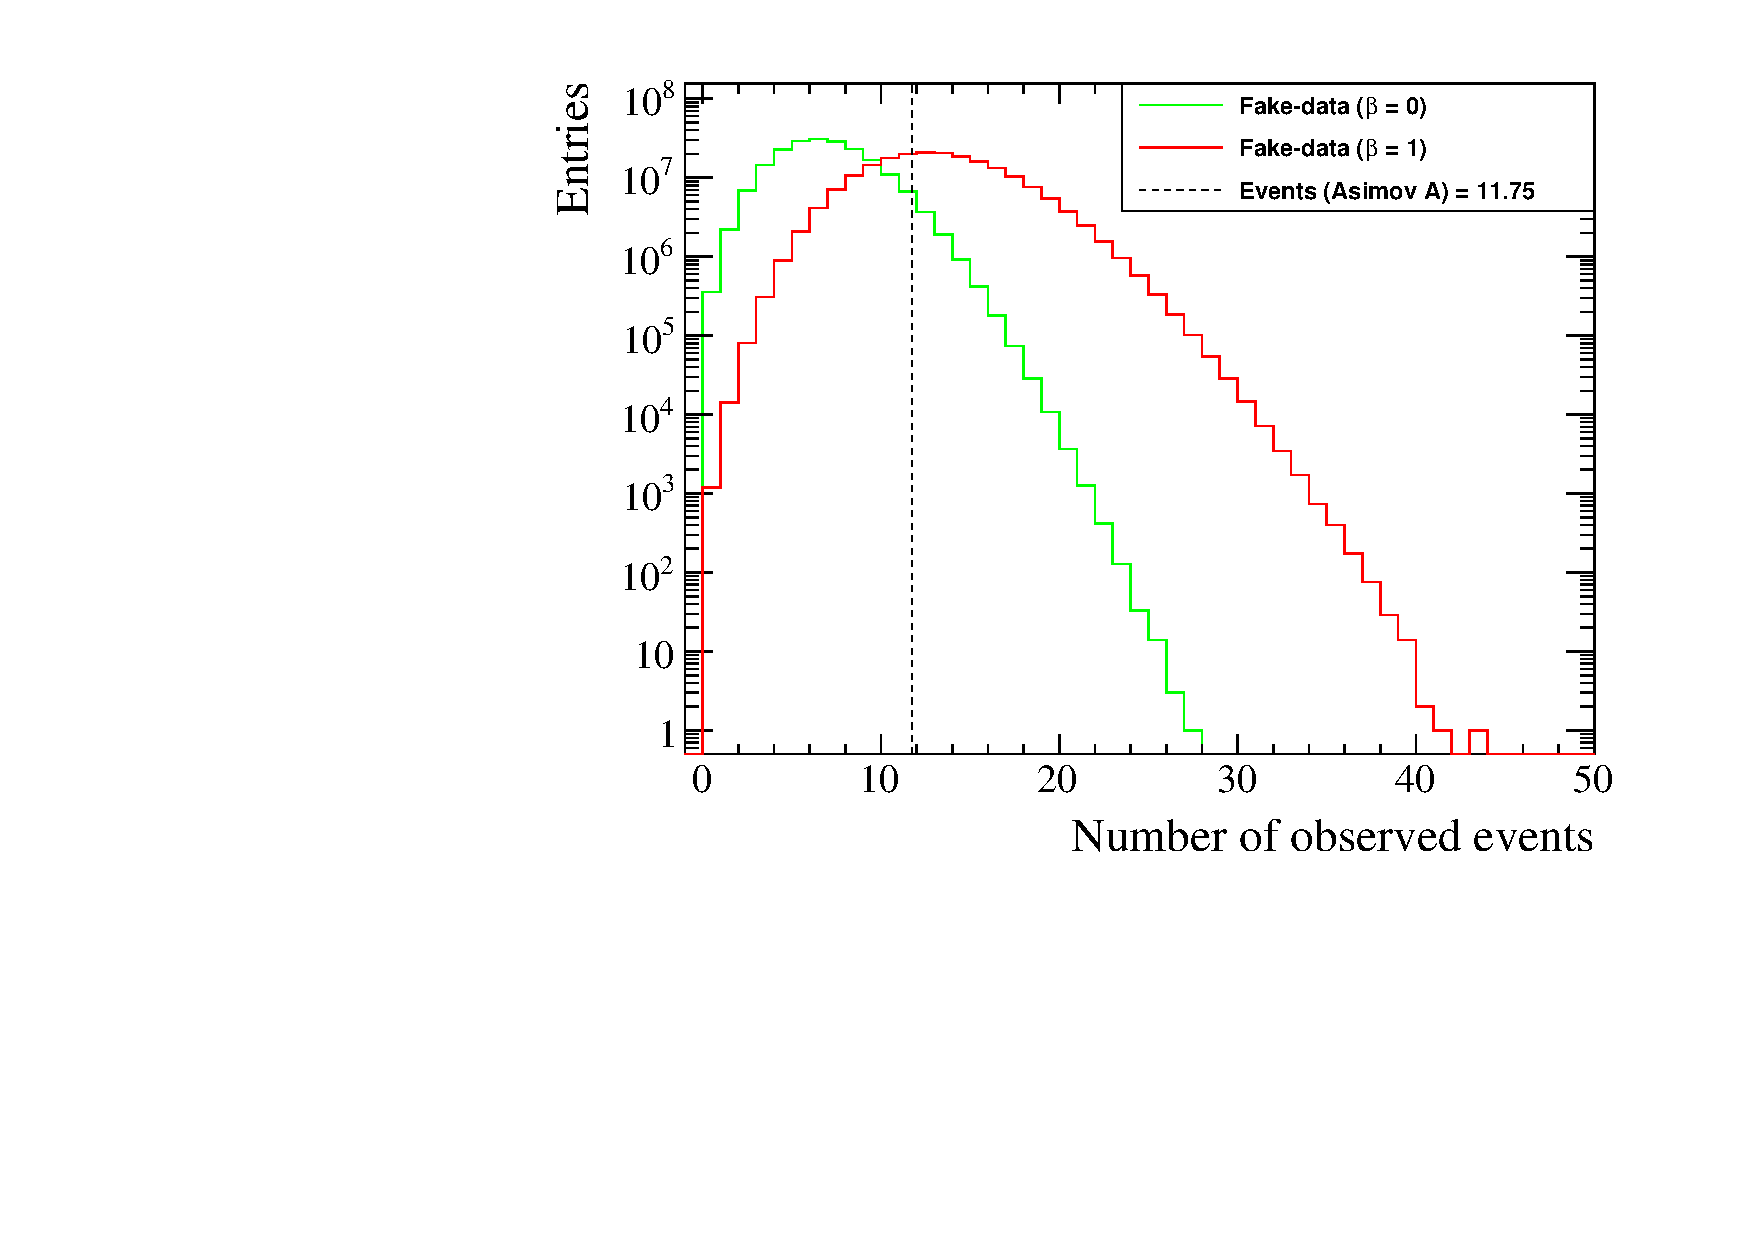
\includegraphics[scale=0.65]{sensitivity/plots_weighted_2018-04-06/rate-only_20ktoys/nuebarapp_graphs_nmargtoys=200k_nexp=20k_rate-only_posterior-predictive_VALORonly_nevents}
	\caption{The distribution of the total number of events in the antineutrino mode single-ring e-like sample from each of the \NToysFakeDataRateOnly\ toy experiments for both the $\beta = 0$ and $\beta = 1$ hypotheses. The distributions were produced using the method outlined in section \ref{sec:method_rate-only} using the Asimov A spectra to calculate the 4-sample likelihood. The dashed line corresponds to the total number of events given by the Asimov A data set.}
	\label{fig:sensitivity_rate-only}
\end{figure}

\begin{figure}
	\centering
	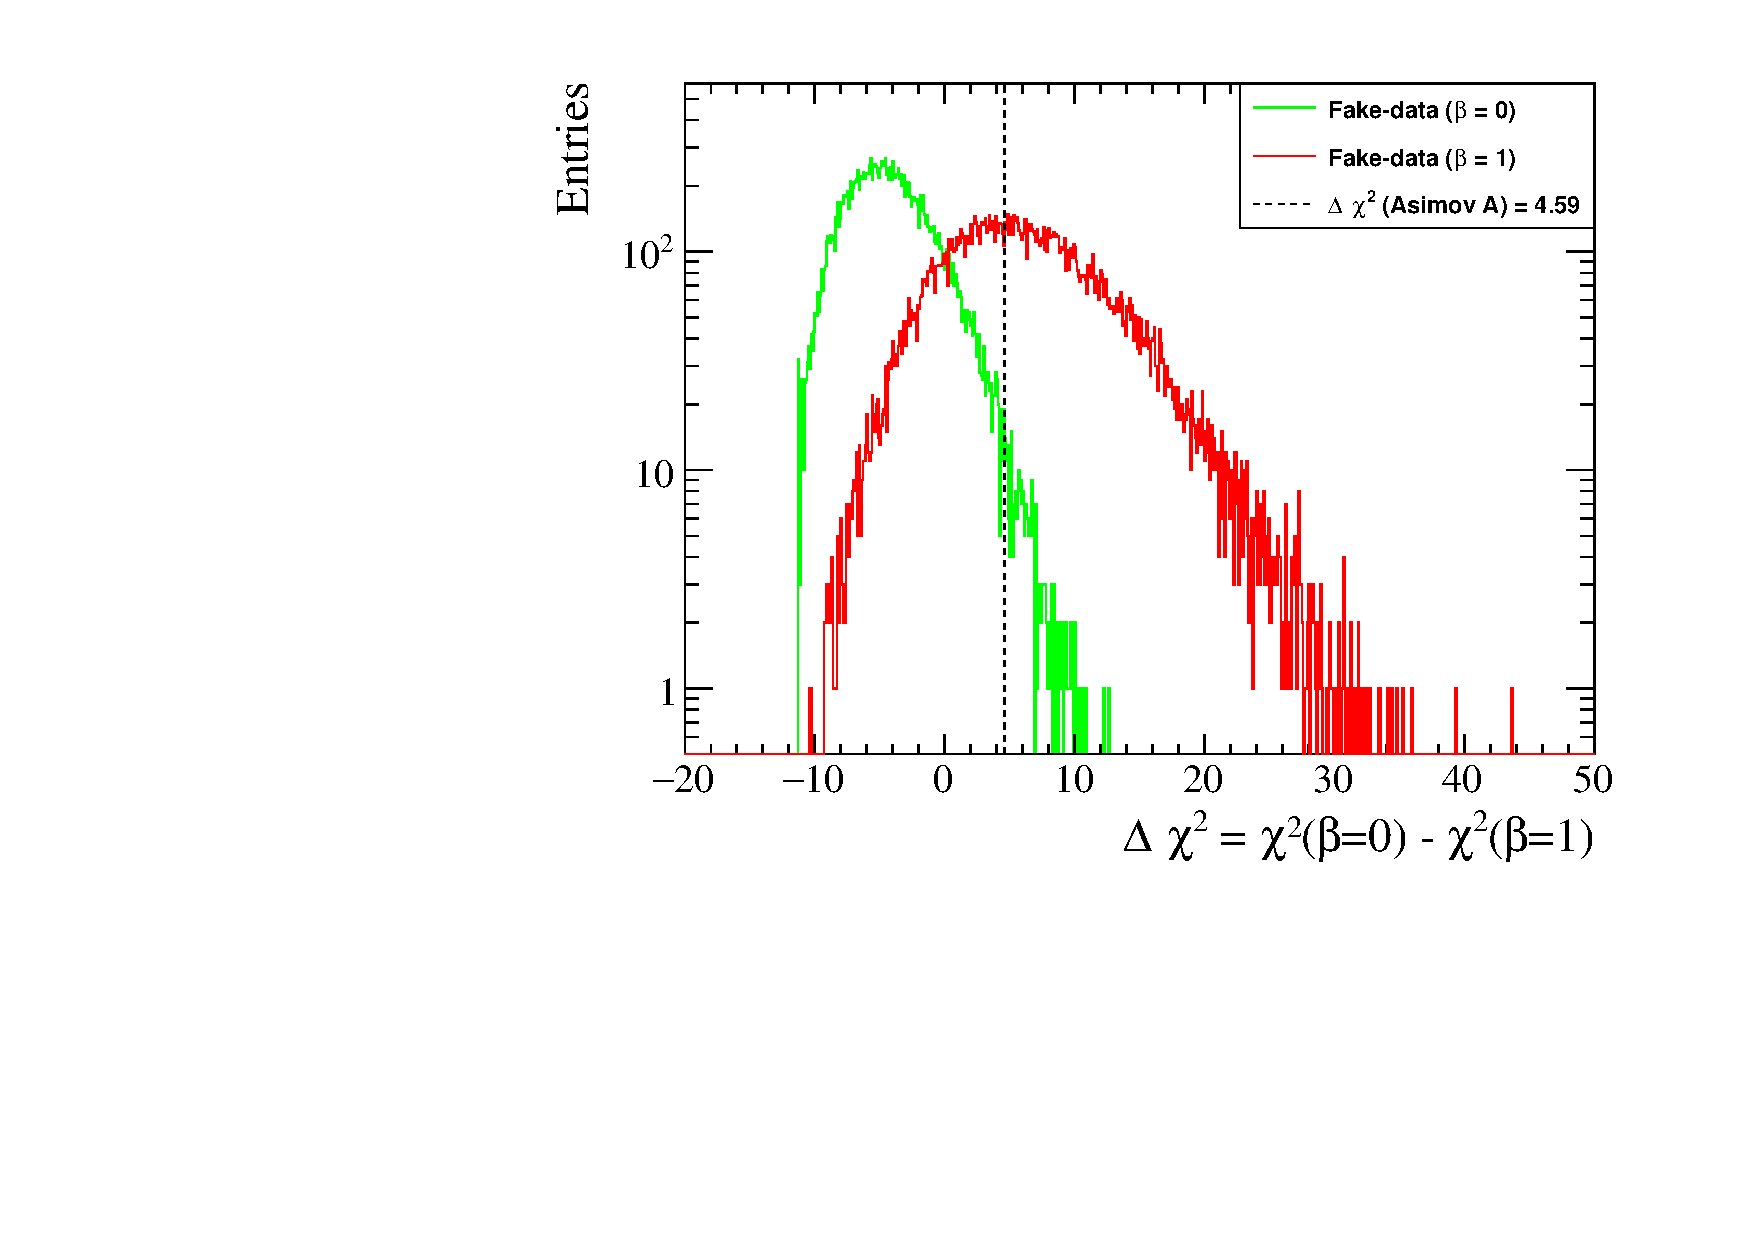
\includegraphics[scale=0.65]{sensitivity/plots_weighted_2018-04-06/rate+shape_20ktoys/nuebarapp_graphs_nmargtoys=200k_nexp=20k_rate+shape_posterior-predictive_VALORonly_Deltachisq_logscale}
	\caption{The distribution of $\Delta \chi^2$ values from each of the \NToysFakeDataRatePlusShape\ toy experiments for both the $\beta = 0$ and $\beta = 1$ hypotheses. The distributions were produced using the method outlined in section \ref{sec:method_rate+shape} using the Asimov A spectra to calculate the 4-sample likelihood. The dashed line corresponds to the $\Delta \chi^2$ value given by the Asimov A data set.}
	\label{fig:sensitivity_rate+shape}
\end{figure}

